\documentclass[10pt, a4paper]{article}
\usepackage[margin=0.35in]{geometry}
\usepackage{fancyhdr}
\usepackage{graphicx}
\usepackage{lscape}
\pagestyle{fancy}
\usepackage{pdfpages}
\lhead{Zack Pollard}
\chead{Object Oriented Programming and Algorithms - Train Route Finder}
\rhead{ID: B424338}
\fancyfoot{}
\setlength{\headheight}{45pt} 
\renewcommand{\headrulewidth}{0.4pt}
\renewcommand{\footrulewidth}{0.4pt}
\graphicspath{{screenshots/}}
\begin{document}
\includepdf[pages={1}]{"Cover Sheet".pdf}
\title{Object Oriented Programming and Algorithms - Train Route Finder}
\author{Zack Pollard}
\maketitle
\section{Design}
I wrote most of my code inside an api package as the code in there had nothing to do with being a CLI. I decided to have the api package as I wasn't sure whether or not I would write a GUI or a CLI at the time, or maybe both. If I had written a GUI as well as a CLI interface, then the API would have ensured that I didn't re-write the generic code. I used an abstract class called Command in order to base all my commands off of this class, this allowed me to have a CommandManager that stored all the commands and I could do lookups and get the objects that I wanted. The class containing the main method for running the CLI is called TrainBookingCLI and it extends TrainBookingAPI in order to inherit it's methods, constructor and also the variables it has.
\section{File format}
The files can be saved with whatever extension is desired by the user. The default file name is main.routes which is created when the program first runs and contains all of the default routes specified in the specification. The routes data is stored using serialisation which Java provides functionality for without any external libraries. Serialisation takes all of the variables in a class and changes them into a format that can be stored to disk. In my case, I serialise the List<Route> of all the routes that are currently loaded. The List is serializable by default and I have made my Route class serializable and so Java can serialize all of the data. This data is not human readable once serialized, but it is stored in such a way that when it is loaded the program can check that the stored data has the same types as the class it is being loaded into, if this is not the case, it will throw an error.
\newpage
\section{UML Diagram for Classes}
\includegraphics[scale=0.65, angle=90]{"UML Diagram".png}
\newpage
\section{Program Testing and Evidence}
\subsection{Input Data Validation}
Here I will show screenshots of me testing the validation checks on data input by the user of my program.

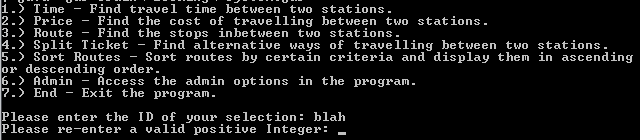
\includegraphics{Validation1.png}

\textit{The screenshot above shows that the program checks to determine if an integer was entered on the main menu.}

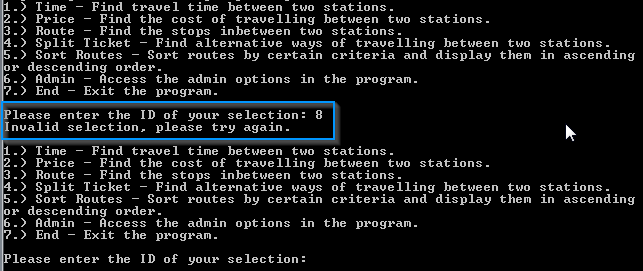
\includegraphics{Validation2.png}

\textit{The screenshot above shows that the program checks to determine if the selection made was a valid option on the main menu.}

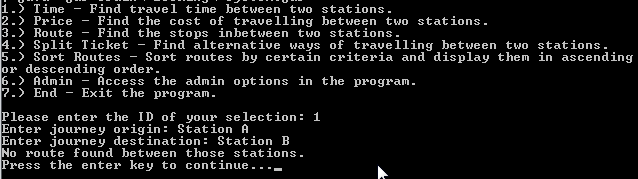
\includegraphics{Validation3.png}

\textit{The screenshot above shows that the program checks to determine if valid stations were entered in the time function.}

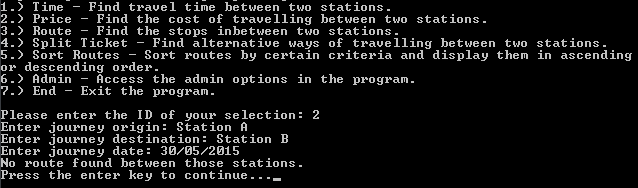
\includegraphics{Validation4.png}

\textit{The screenshot above shows that the program checks to determine if valid stations were entered in the price function.}

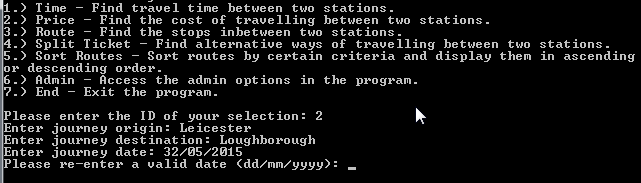
\includegraphics{Validation5.png}

\textit{The screenshot above shows that the program checks to determine if a valid date was entered in the price function.}

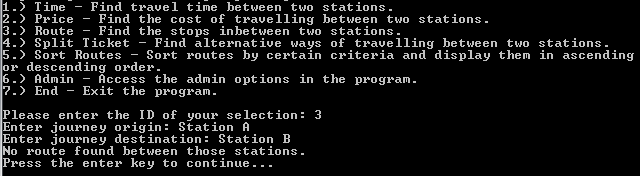
\includegraphics{Validation6.png}

\textit{The screenshot above shows that the program checks to determine if valid stations were entered in the route function.}

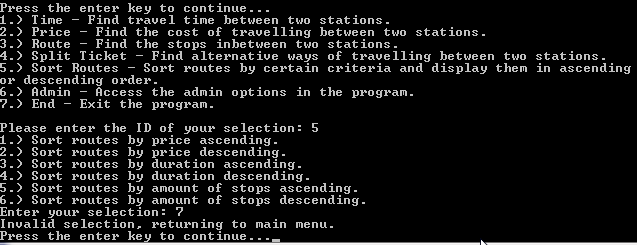
\includegraphics{Validation7.png}

\textit{The screenshot above shows that the program checks to determine if the selection made was a valid option on the sorting selection menu.}

\subsection{Functionality Testing}

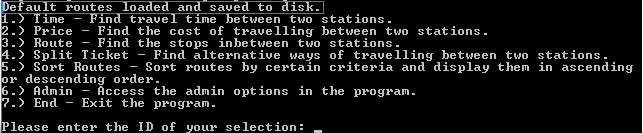
\includegraphics{Functionality1.png}

\textit{The screenshot above shows that the default routes are loaded and saved to the default file location when no routes file exists on startup.}

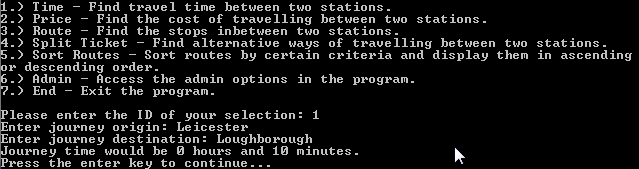
\includegraphics{Functionality2.png}

\textit{The screenshot above shows that the time function works as expected.}

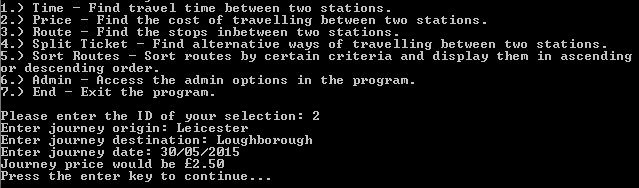
\includegraphics{Functionality3.png}

\textit{The screenshot above shows that the price function works as expected.}

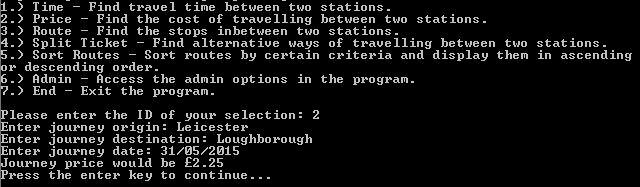
\includegraphics{Functionality4.png}

\textit{The screenshot above shows that the price function takes into account the last day of the month and offers a discount.}

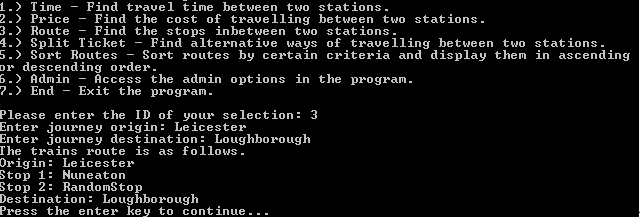
\includegraphics{Functionality5.png}

\textit{The screenshot above shows that the route function works as expected.}

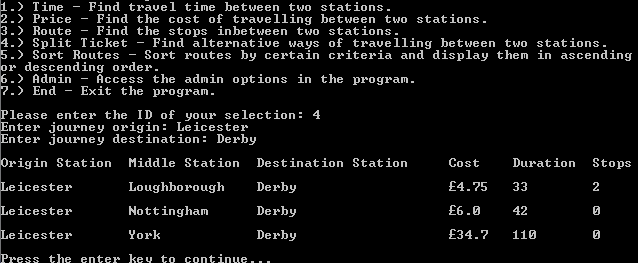
\includegraphics{Functionality6.png}

\textit{The screenshot above shows that the split ticket function works as expected.}

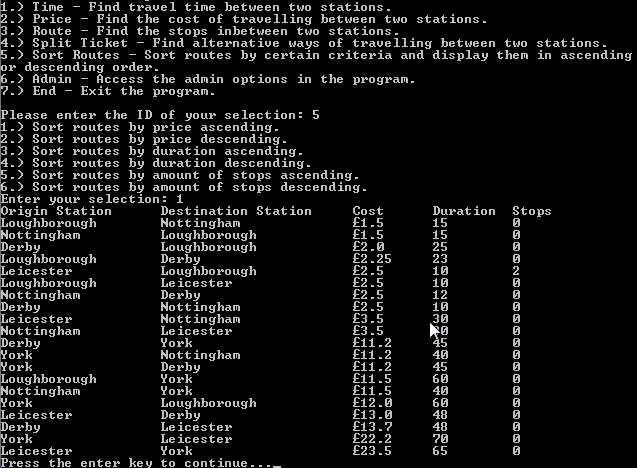
\includegraphics{Functionality7.png}

\textit{The screenshot above shows that the sort routes function works as expected for price ascending.}

\newpage
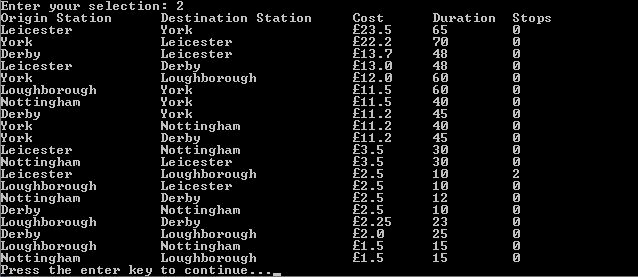
\includegraphics{Functionality8.png}

\textit{The screenshot above shows that the sort routes function works as expected for price descending.}

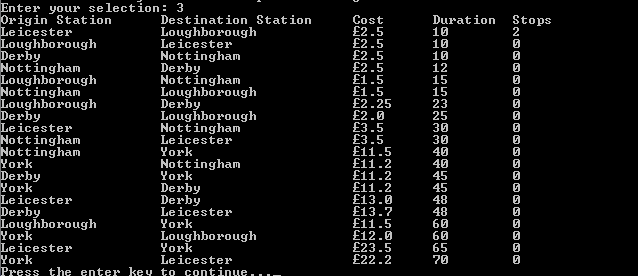
\includegraphics{Functionality9.png}

\textit{The screenshot above shows that the sort routes function works as expected for duration ascending.}

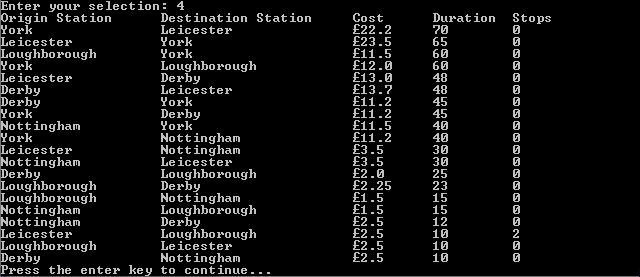
\includegraphics{Functionality10.png}

\textit{The screenshot above shows that the sort routes function works as expected for duration descending.}

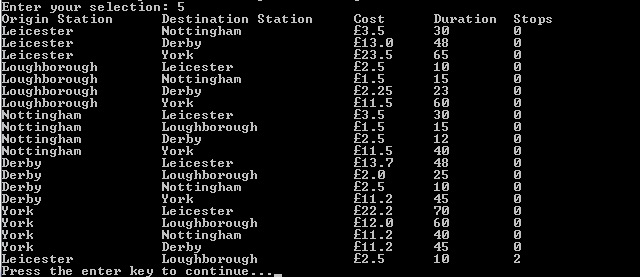
\includegraphics{Functionality11.png}

\textit{The screenshot above shows that the sort routes function works as expected for routes ascending.}

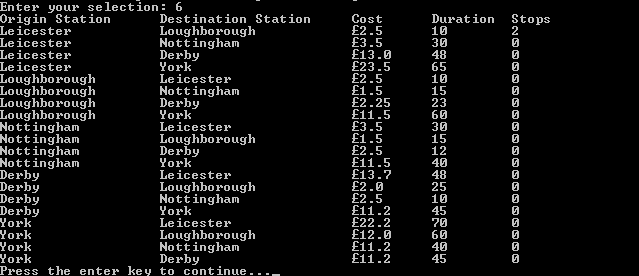
\includegraphics{Functionality12.png}

\textit{The screenshot above shows that the sort routes function works as expected for routes descending.}

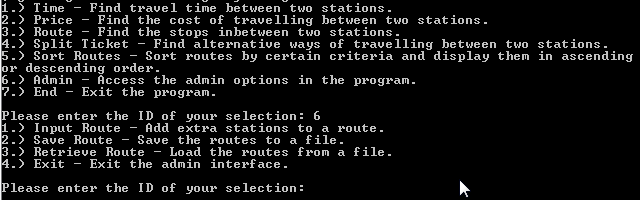
\includegraphics{Functionality13.png}

\textit{The screenshot above shows that the admin menu loads when you select it from the main menu.}

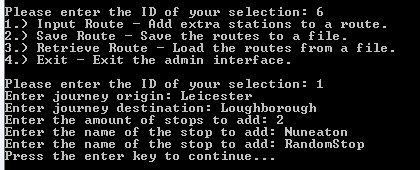
\includegraphics{Functionality14.png}

\textit{The screenshot above shows that the input route function works as expected.}

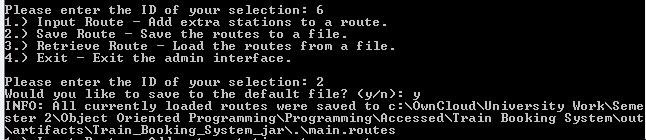
\includegraphics{Functionality15.png}

\textit{The screenshot above shows that the save routes function works for saving to the default file.}

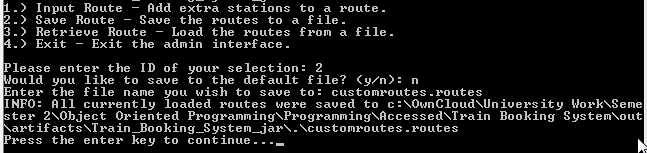
\includegraphics{Functionality16.png}

\textit{The screenshot above shows that the save routes function works for saving to a custom file.}

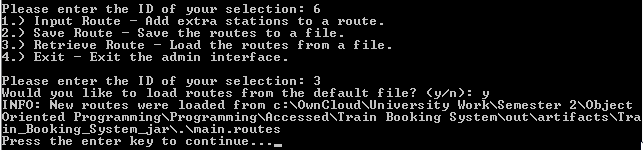
\includegraphics{Functionality17.png}

\textit{The screenshot above shows that the retrieve routes function works for loading from the default file.}

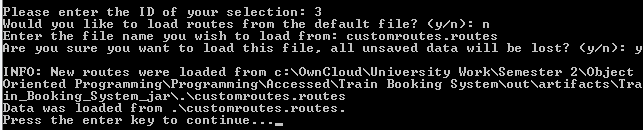
\includegraphics{Functionality18.png}

\textit{The screenshot above shows that the retrieve routes function works for loading from a custom routes file.}

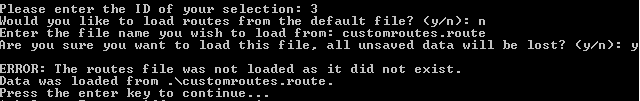
\includegraphics{Functionality19.png}

\textit{The screenshot above shows that the retrieve routes function detects if the file does not exist when requested for loading.}

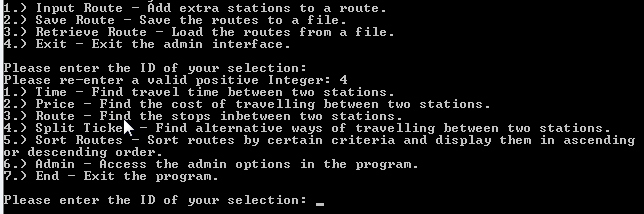
\includegraphics{Functionality20.png}

\textit{The screenshot above shows that the exit option works and returns to the previous menu.}

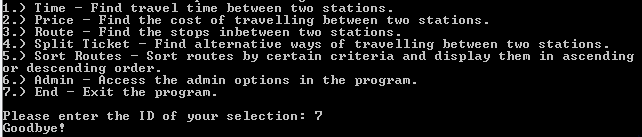
\includegraphics{Functionality21.png}

\textit{The screenshot above shows that the end option works and exits the program.}


\section{Functionality}
\begin{table}[h]
\begin{tabular}{|p{125pt} | p{60pt} | p{300pt}|}
\hline
\textbf{Functionality} & \textbf{Y(Complete) P(Partial) N(None)} & \textbf{Comments (e.g. more details on what is not working etc.)} \\ \hline
Search for price & Y & \\ \hline
Search for travel time & Y & \\ \hline
Display route & Y & \\ \hline
Split ticket & Y & Displayed a list of all available split routes as was unsure on what was required. \\ \hline
Sort route data & Y & I provided the option of sorting it ascending and descending as I wasn't sure if you wanted one or both. \\ \hline
Input route & Y & \\ \hline
Load route (from file) & Y & \\ \hline
Save route (to file) & Y & \\ \hline
Handling dates correctly & Y & \\ \hline
Error handling & Y & All errors that could be a problem are handled by the Logger and will be printed out to console with both the stacktrace and an informative message as to what went wrong.\\ \hline
\end{tabular}
\end{table}
\end{document}